%!TEX root = ../main.tex
\chapter{Literature Review}
\label{chap:litReview}

\section{Gamification}
\subsection{Defining Gamifaction}
Gamification is attempted to be defined by \cite{Deterding:2011:GDE:2181037.2181040} as ``The use of design elements for games in non-game contexts''. 
A game design element is referred to as the characteristics of a game that appear in most games, readily associated with games and are found to play a significant role in games.
With this definition, it is necessary to identify what the game design elements that will be included in the application will be. 

In this paper, Deterding also highlights the fact that Gamification refers specifically to using game elements in a non-game application, rather than using full-fledged games.
It could be argued by this strict definition that my application is not true gamification as it is built as a full game.
However, in return it could be said that my application - at it's core - is a task management application that incorporates RPG game elements.

\cite{huotari2011gamification} have provided an alternative definition for gamification, stating that it is ``service packaging where a core service is enhanced by a rules-based service system that provides feedback and interaction mechanisms to the user with an aim to facilitate and support the users’ overall value creation.''


\subsection{Rewards and Punishments}
In an experiment by \cite{Filsecker2014136}, children were separated into two groups - a public recognition (PR) group where the childs `badges' were recorded on a leaderboard placed prominently in a room where others can see, and a non-public recognition (NPR) group.
The children were then given an educational game called Taiga which would ask them to pose a hypothesis as to why the number of fish in a pond had been decreasing over time, and then perform experiments to justify or disprove the hypothesis.
It was found that students achieved a statistically significant increase in understanding and performance of topics in the PR group compared to the NPR group.
Taiga had a variety of educational content embedded within the game that the users can access, and tracked which ones the children had checked during the tasks to determine whether the children were motivated to access more of these. 
It was then found that the PR group did not access any more of these educational materials than the NPR group, which was unexpected given the previous findings. 
The badges awarded by Taiga are synonymous with the common game design element of `Achievements', which are awarded to the user after a certain set of requirements have been met - e.g. Achievement Unlocked - Complete 10 Quests.

A common issue with rewards in education is that ``extrinsic'' rewards (rewards not relating to the activity they are awarded for) ultimately end up undermining the child's attention and motivation from the intrinsic learning activity once the rewards are removed \citep{deci2001extrinsic,ACP:ACP2350090502}.
This diminishes the usefulness of rewards as a long-term motivation for children.
However, \cite{cameron2001negative} highlights that this effect only occurs with children who had high initial interest in the task at hand. 
For example, rewarding a child for performing in his favourite sport only serves to undermine their original interest in the sport.

\cite{deci2001extrinsic} also found that unexpected rewards had the least negative impact and highest positive effect for children's attention in a task. 
This could mean that it would be beneficial to include an element of randomness to the rewards for completing a task, such as a random chance of earning an item for each quest.


\section{Game Design}
\subsection{Game Design Elements}
\cite{Deterding:2011:GDE:2181037.2181040} separated game design elements into five different levels as shown in figure \ref{fig:GameDesignElements}. 
The key elements I will focus on in my application are `Game interface design patterns', which are common components in games that are not specifically `played with' themselves, but run alongside a game to increase offer more feedback or fun in the application.
This includes elements such as badges/acheivements, leaderboards, levels and experience points.

\begin{figure}[ht]
	\centering
	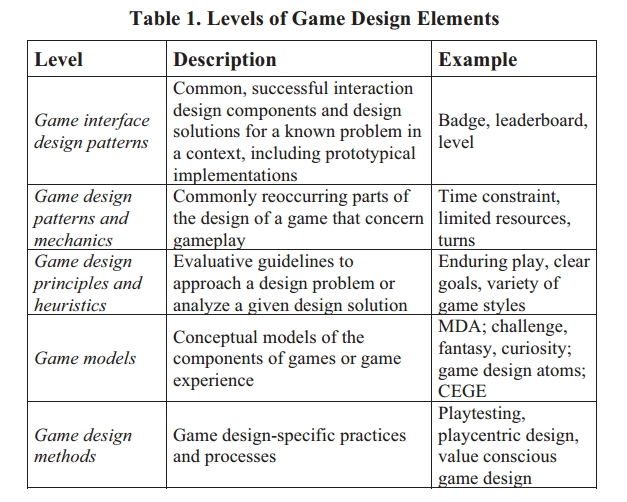
\includegraphics[scale=0.45]{images/DeterdingsLevelsOfGameDesignElements.jpg}
	\caption{Levels of Game Design Elements}
	\label{fig:GameDesignElements}
\end{figure}

As previously mentioned, it is important to specify what game design elements I will choose to use in my application.
In the book `100 Elements of Game Design' \citep{despain2012100}, it mentions several useful elements to use.

\subsubsection{Achievements}
Achievements are defined by \cite{Montola:2009:AGA:1621841.1621859} as ``optional sub-goals in a secondary reward system''. 
They are also described as being separate to the core game system and do not affect the progress of the player, and should be seen as more of a meta-game. Achievement features are one of the most commonly implemented game design patterns in gamification \citep{hamari2011framework}.

\cite{Montola:2009:AGA:1621841.1621859} raised concerns in regards to applying achievements to non-game applications that they would create unproductive or unintended behaviours by users. 
For example, an achievement on a forum for making 1000 posts may inadvertently motivate users to make a large amount of low-effort or spam posts, reducing the quality of the forum.
However, \cite{Montola:2009:AGA:1621841.1621859} also noted that some users appreciated the changes and found the achievements to be motivating. 

\subsubsection{Character Development}

\subsubsection{Rewards}
\cite{king2010video} lists a variety of different reward structures in video games, such as in-game currency, experience points, levelling up and `rare-item' rewards. 
As the tasks in KidQuest are structured as Role-Playing Game (RPG) quests, there already exists well established methods of rewarding the user. 
In RPGs, quests often have these key reward structures and therefore are established to work suitably well for KidQuest.

The rate at which these rewards are earned must be examined to ensure they still feel rewarding throughout. 
For example, if a quest returns 100 XP points and you require 300 XP to level up from level 1 to 2, this only requires you to complete three quests to level up, meaning these three quests feel rewarding as each quest is offering 1/3rd of a level.
However, the XP if quests still offer 100 XP and you require 6000 XP to level up from level 30 to 31, the reward from the same quest is now worth 1/60th of a level, despite being the same difficulty to the user.
Therefore, some scaling of the rewards is required in the app to allow XP rewards to scale suitably with the XP required to level.
This scaling is referred to as `increasing cost' \citep{1_anderson_2016}.
Anderson also shows that it is important to determine reasonable caps for numerical relationships in video-games, to stop the increasing cost becoming out of proportion.

\cite{1_anderson_2016} poses that a useful pattern for these kinds of relationships is a classic triangular pattern, in which the first level requires 1 XP to level up, the second level requires 3 XP, the third requires 6. To allow for more meaningful numbers to the user, I have multiplied the results of the formula by 100.

\begin{equation} \label{eq:xprequiredfornextlevel}
	T_n= \frac{n(n+1)}{2} \times 100
\end{equation}

Initially, the scaling formula for XP rewards involved using 60XP as a base reward for a medium difficulty quest, then using the player's current level, it would derive a multiplier that would be used to scale the XP reward.
\begin{equation} \label{eq:xpgainedlinear}
	\textrm{XP Gained} = 60 \times \frac{(n - 1) \times k}{100} + 1
\end{equation}
Where k can be adjusted to specify the strength of the multiplier against the XP rewards, so that if k = 10, a character at level 31 would have a 3x multiplier on quests, meaning the same quest that gave them 60XP at level 1, now gives them 180XP.
However, when modelling this equation, the number of quests completed quickly becomes out of hand. 
At level 1, the player must complete 2 medium quests to level up - a reasonable starting point.
However by level 25 the player must complete 22 quests to level up and by level 99 (One before the level cap) the player must complete an extraordinary 84 medium difficulty quests to level up.

Therefore, triangular numbers can also be useful for calculating the XP gained per quest. By adjusting the triangular numbers formula somewhat, I found a suitable middle ground which still gives the new user the feeling of progressing quickly, but the rate of quests per level quickly slows down to a limit of approximately 10 quests per level by level 100.
This will ensure that the player will still feel like they are progressing at a reasonable speed throughout.

\begin{equation} \label{eq:xpgainedtriangular}
	\textrm{XP Gained} = \frac{(n+2)(n+3)}{2} \times 10
\end{equation}


%TODO: Work out wtf you are doing with this chart
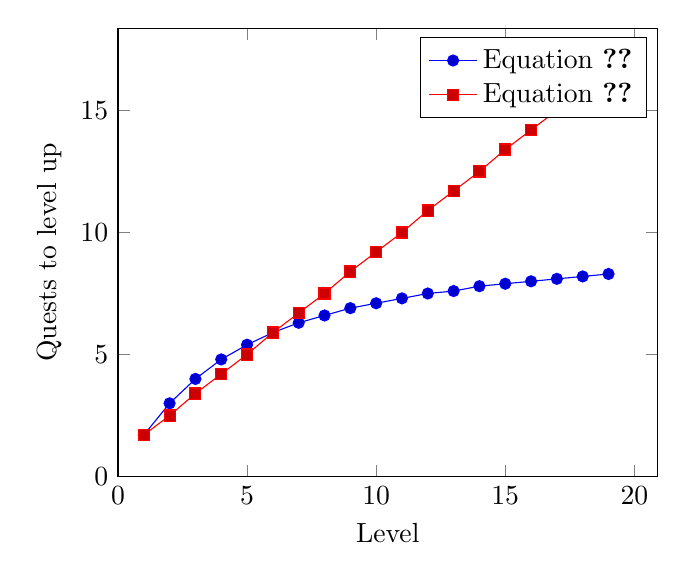
\begin{tikzpicture}	
	\begin{axis}[
		xlabel=Level,
		ylabel=Quests to level up,
		xmin=0,
		ymin=0,
	]
		\addplot coordinates {
			(1, 1.7)
			(2, 3)
			(3, 4)
			(4, 4.8)
			(5, 5.4)
			(6, 5.9)
			(7, 6.3)
			(8, 6.6)
			(9, 6.9)
			(10,7.1)
			(11,7.3)
			(12,7.5)
			(13,7.6)
			(14,7.8)
			(15,7.9)
			(16,8)
			(17,8.1)
			(18,8.2)
			(19,8.3)
		};
		\addlegendentry{Equation \ref{eq:xpgainedtriangular}}
		\addplot coordinates{
			(1, 1.7)
			(2, 2.5)
			(3, 3.4)
			(4, 4.2)
			(5, 5)
			(6, 5.9)
			(7, 6.7)
			(8, 7.5)
			(9, 8.4)
			(10, 9.2)
			(11, 10)
			(12, 10.9)
			(13, 11.7)
			(14, 12.5)
			(15, 13.4)
			(16, 14.2)
			(17, 15)
			(18, 15.9)
			(19, 16.7)
		};
		\addlegendentry{Equation \ref{eq:xpgainedlinear}}
	\end{axis}
\end{tikzpicture}


\subsubsection{Feedback Loops}
A positive feedback loop involves the player becoming more powerful throughout the game, which in turn makes things easier to complete, which means they can complete more quests and become more powerful even quicker.
Whilst this sounds like a good element to the game, it is important that developers avoid allowing this to destabilise the game, by making quests - and therefore the game - trivial.
As in my application, quests are completed in the real world and are not tied into the in-game character's power, I will be largely unaffected by this.
However, if I seek to include an element of competitiveness into the game by allowing users to `battle' each other, it is important to take steps to avoid players becoming too powerful that the battles are no longer enjoyable.

\subsubsection{Competitiveness}

\subsection{Educational Games}
\cite{Denis:2005:MEG:1178477.1178581} draws a stark contrast between the motivation levels in education and video games, highlighting how 	

\section{Smartphone Applications}


\subsection{Android vs. iOS}
When planning the development of a mobile application, it must be considered which platform is best to target. 

\subsubsection{Market Share}
Figure \ref{fig:PhoneMarketShare} clearly shows Android's strong hold over the global market share, holding over 70\% of units shipped since Q3 of 2012. 
Meanwhile, figure \ref{fig:UKPhoneMarketShare} also shows an Android dominance in the UK market specifically, however the hold over the market is less strong at 57\% in 2014 and 52\% in 2015, and shows a downward trend in the market share of Android.

\begin{figure}[ht]
	\centering
	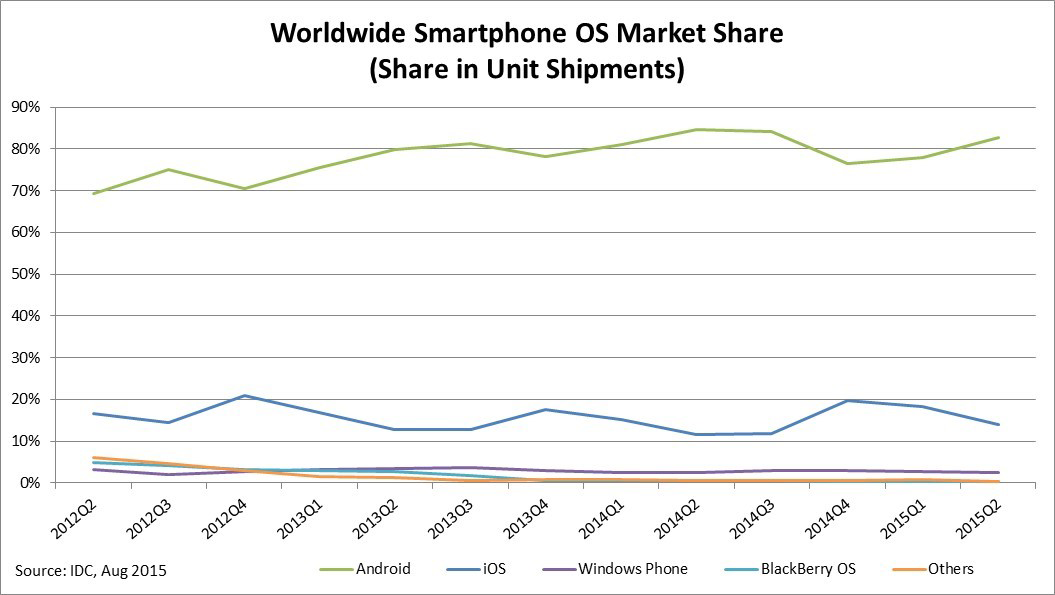
\includegraphics[scale=0.65]{images/phoneMarketShare.png}
	\caption{Worldwide Smartphone OS Market Share \citep{idcsmartphonereport}}
	\label{fig:PhoneMarketShare}
\end{figure}

\begin{figure}[ht]
	\centering
	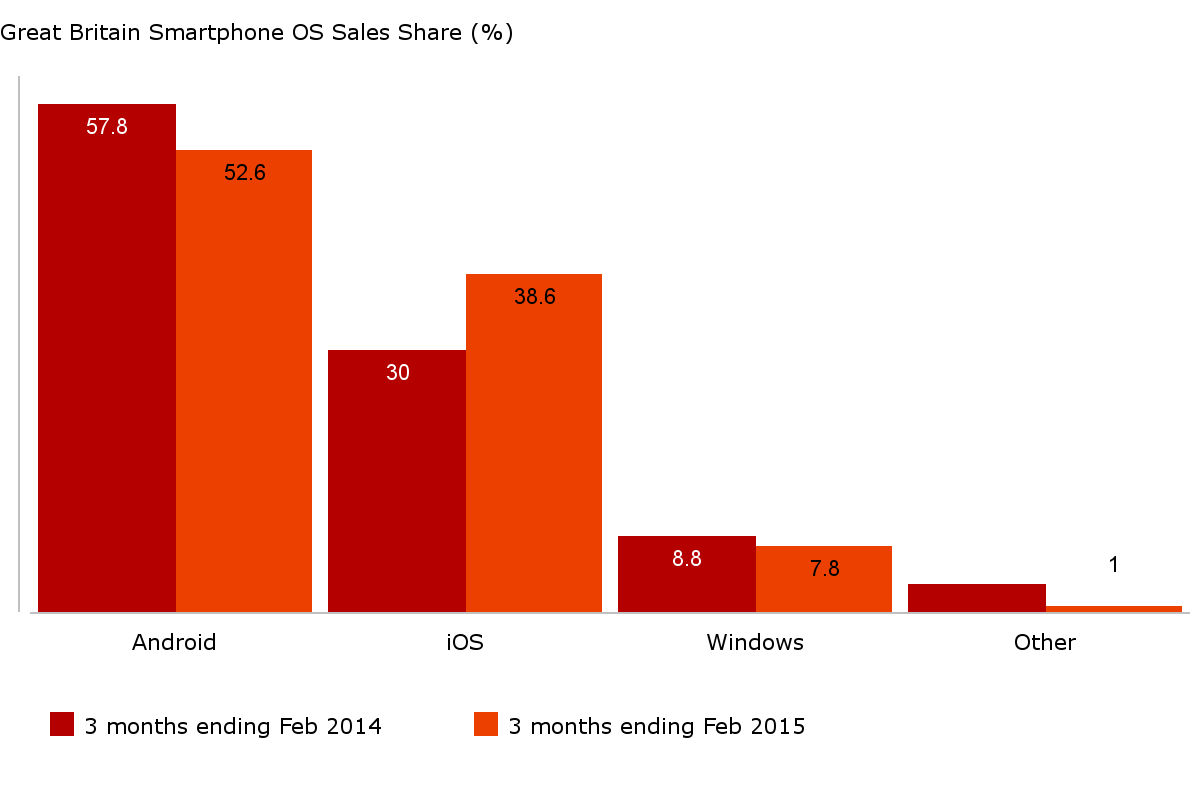
\includegraphics[scale=0.25]{images/UKSmartphoneSales.png}
	\caption{Great Britain Smartphone OS Market Share \citep{kantargbsmartphonereport}}
	\label{fig:UKPhoneMarketShare}
\end{figure}

\subsubsection{Fragmentation}
A common issue with developing for mobiles is that many people do not (or cannot) update their devices to the latest versions.
Android in particular is problematic for this, as shown in figure \ref{fig:AndroidVersions}.
This problem is referred to as `Fragmentation'.
Despite being released in October of 2015, the latest Android version Marshmallow is still at less than 2.5\% adoption rate. 
This is primarily due to software updates being held back by network carrier locked phones and phones falling out of support.

\begin{figure}[ht]
	\centering
	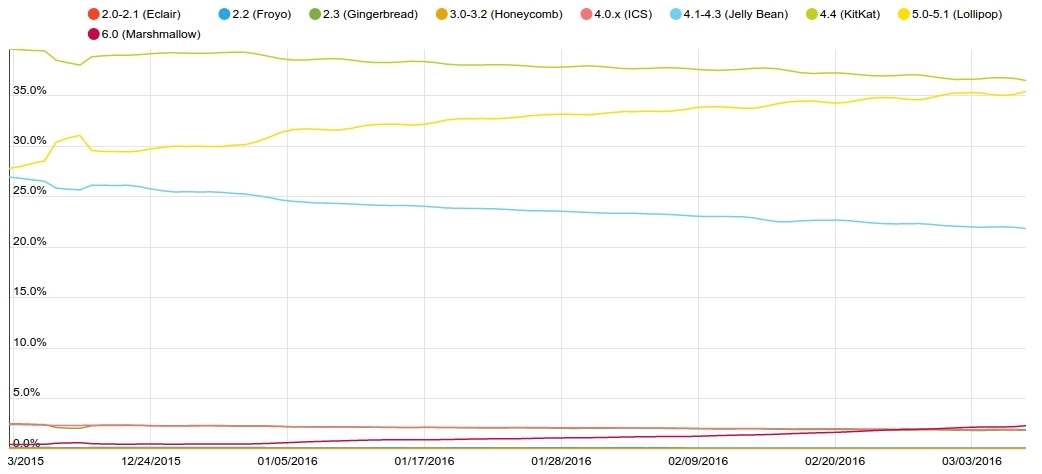
\includegraphics[scale=0.4]{images/AndroidSDKMarketShare.jpg}
	\caption{Android SDK Market Share \citep{appbrainsdkversions}}
	\label{fig:AndroidVersions}
\end{figure}

As Android phones are manufactured by a variety of different companies, there is less standardization between available handsets. 
\cite{uniqueandroiddevices} reported that it detected nearly 24,100 distinct devices that downloaded its app in 2015.
This shows just how much of a problem fragmentation could pose to Android development.

This also leads to concerns about the variety of screen sizes in these devices, as apps will have to be designed and maintained to support a myriad phones. 
However, \cite{androidscreenfragmentation} shows that due to the similarities of resolutions between these phones, there are only four key resolutions that need to be managed within Android.